\documentclass[conference]{IEEEtran}
\IEEEoverridecommandlockouts
% The preceding line is only needed to identify funding in the first footnote. If that is unneeded, please comment it out.
\usepackage{cite}
\usepackage{amsmath,amssymb,amsfonts}
\usepackage{algorithmic}
\usepackage{graphicx}
\usepackage{textcomp}
\usepackage{xcolor}
\def\BibTeX{{\rm B\kern-.05em{\sc i\kern-.025em b}\kern-.08em
    T\kern-.1667em\lower.7ex\hbox{E}\kern-.125emX}}

\begin{document}

\title{Skin Cancer Classification Using Deep Learning\\}
\author{\IEEEauthorblockN{Dwarkanath Prabhu}
\IEEEauthorblockA{\textit{Department of Industrial and Systems Engineering)} \\
\textit{Texas A\&M University}\\
College Station, TX, USA \\
pdwarkanath@tamu.edu}
\and
\IEEEauthorblockN{Xiaoning Qian}
\IEEEauthorblockA{\textit{Department of Electrical and Computer Engineering} \\
\textit{Texas A\&M University}\\
College Station, TX, USA \\
xqian@tamu.edu}
}

\maketitle

\begin{abstract}
\textbf{The ISIC Challenge 2018 consists of 3 tasks. This report is aimed at tackling Task 3 - Disease Classification from images of skin lesions. VGG19, ResNet50, Inceptionv3, SqueezeNet, pretrained on ImageNet, were chosen as models for this purpose. Only the last 2 layers were retrained for these models on the ISIC dataset. The best performing model was selected which turned out to be ResNet50. The class imbalance in the training data was dealt with using a class-weighted loss function and oversampling of low frequency classes.}
\end{abstract}

\section{Introduction}\label{introduction}

In the United States, 5 million new cases of skin cancer are diagnosed
every year.\cite{rogers2015incidence} Of these, melanoma which is the deadliest accounts
for over 9000.\cite{siegel2017cancer} The diagnosis via visual inspection by patients
and dermatologists is accurate only about 60\% of the time.\cite{kittler2002diagnostic}
Moreover, the shortage of dermatologists per capita has abetted the need
for computer-aided methods to detect skin cancer.\cite{kimball2008us}

The International Skin Imaging Collaboration (ISIC) has aggregated a
large amount of publicly accessible dermoscopy images labeled with
ground truth data. The ISIC 2018 challenge \cite{codella2018skin} was divided into 3
tasks - Task1: Lesion Segmentation, Task 2: Lesion Attribute Detection
and Task 3: Disease Classification. This report focuses on Task 3 i.e.
classification of images into one of 7 possible classes.

    \section{Dataset}\label{dataset}

There are 10,015 images in the labeled training dataset.\cite{tschandl2018ham10000} Some sample
images from the dataset and their labels are shown in Fig \ref{fig1}. The labels are stored in a CSV file in the form of stacked transposes of one-hot vectors. i.e. each example in the dataset is represented by a row of length 7 with only the class to which the exmple belogns being 1 and the other elements in the row being 0. There are no missing
labels and all images are classified into one of 7 classes: 
\begin{itemize}
\item Melanoma
\item Melanocytic nevus 
\item Basal cell carcinoma
\item Actinic keratosis / Bowen's disease (intraepithelial carcinoma)
\item Benign keratosis (solar lentigo / seborrheic keratosis / lichen planus-like keratosis) 
\item Dermatofibroma
\item Vascular lesion
\end{itemize}

\begin{figure}[htbp]
\centerline{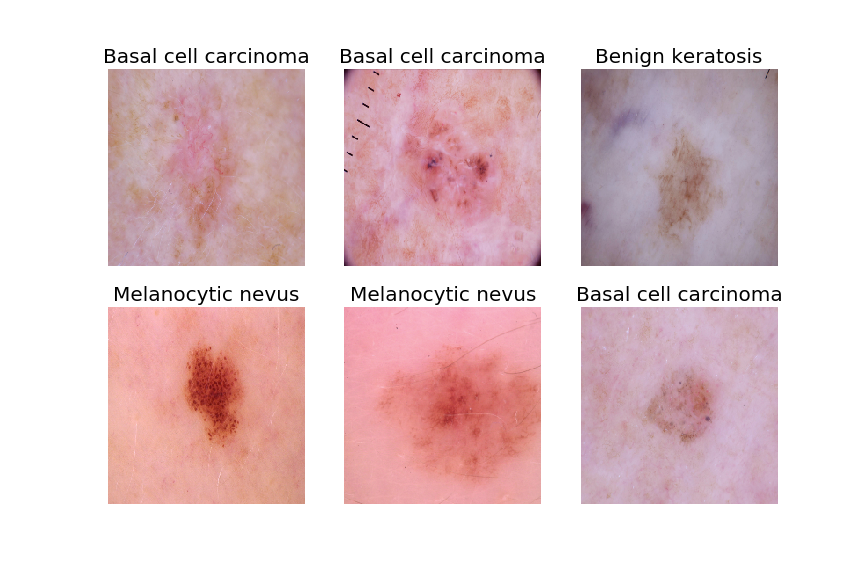
\includegraphics[width=\columnwidth]{Task3-Imgs.png}}
\caption{Sample Images from Task 3 Dataset with Labels}
\label{fig1}
\end{figure}

 Evaluation metric for this task is the multi-class accuracy (MCA) i.e. the average of precision for all classes. Eq \ref{eq1} shows the calculation for the MCA.

\begin{equation}
MCA = \frac{1}{n}\sum_{i=0}^{n-1}{P_i}
\label{eq1}
\end{equation}

where $P_i$ is the precision of class $i$ and $n$ is the number of classes


    \section{Architecture}\label{architecture}

Since this is a problem of image classification, a convolutional neural
network (CNN) architecture would be most suitable. We used existing
models such as VGG19\cite{simonyan2014deep}, SqueezeNet\cite{DBLP:journals/corr/IandolaMAHDK16}, Resnet50\cite{DBLP:journals/corr/HeZRS15},
Inception\cite{DBLP:journals/corr/SzegedyLJSRAEVR14} with weights pretrained on ImageNet\cite{russakovsky2015imagenet}\cite{lee2017tensornets}. 
Since ImageNet uses an input size of 224x224 and the images in the
dataset are 450x600, the first step was to scale the images down to the
required 224x224 size (except Inception which requires an input size of 299x299). 
Finally, the last few layers of each model were removed and replaced with 2 fully connected trainable layers. 
First layer trained has 120 units with ReLU activation and the second, a softmax classifier with 7 output classes. 
A randomly selected sample of 10\% of the dataset was used as a validation set to calculate the MCA and compare the models.

The number of layers removed and results achieved from these architectures is shown in Table \ref{tab1}. As it can be seen the simpler models (VGG19 and SqueezeNet) performed poorly on the dataset but more sophisticated models (ResNet50 and Inception) performed better. Since, ResNet50 achieved the best performance on the evaluation metric, it was chosen for further improvement.


\begin{table}[htbp]
\caption{Architecture Performance}
\begin{center}
\begin{tabular}{|l|c|c|}
\hline
\textbf{Architecture} & \textbf{Layers Removed} & \textbf{Validation MCA}\\
\hline
VGG19 & 2 & 9.57\%\\
\hline
SqueezeNet & 2 & 9.57\%\\
\hline
ResNet50 & 3 & 62.74\%\\
\hline
Inceptionv3 & 3 & 54.37\%\\
\hline
\end{tabular}
\label{tab1}
\end{center}
\end{table}

    \section{Improving Performance}\label{improving-performance}

Approximately 70\% of the images belong to only one class (Melanocytic
nevus). Hence, it is trivial to achieve around 70\% accuracy by simply
predicting all images to be of that class. That is obviously incorrect.
In order to improve performance, we try several techniques such as data
augmentation, oversampling low-frequency classes, weighted loss etc.

As expected a baseline ResNet50 model achieved a validation MCA of only 62.74\% MCA while the
training MCA was 93.67\%. We will attempt to improve this discrepancy in
the performance of training and validation set by using some techniques
as follows.

\begin{figure}[htbp]
\centerline{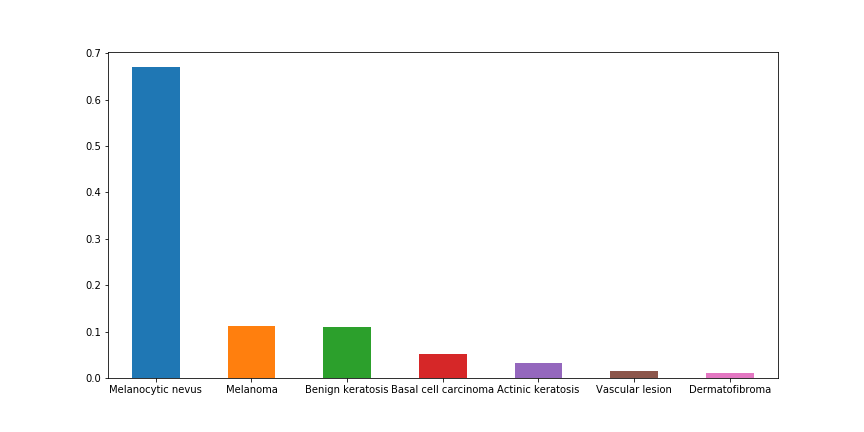
\includegraphics[width=\columnwidth]{Task3-DiseaseTypeFrequency.png}}
\caption{Distribution of classes in the training set }
\label{fig2}
\end{figure}



    \subsection{Batch Normalization}\label{batch-normalization}

Since we are using ReLU activation in the fully connected layers and
the final output is a softmax i.e. a number between 0 and 1, batch
normalization \cite{ioffe2015batch} could help speed up training by scaling the
output of the fully connected layers appropriately. The performance on
the validation set improved slightly to 73.29\% but the training MCA
went down to 87.77\%.

\subsection{Data Augmentation -
Mirroring}\label{data-augmentation---mirroring}

There is still a large difference between the validation and training
MCA. Training the model on a larger dataset could help bridge this gap.
We can double the dataset by simply taking mirror images \cite{NIPS2012_4824} of the
existing dataset while keeping the labels constant. Training the model on the dataset with original imges and their horizontal mirror images increased the validation MCA to 76.27\% while the training MCA was up to 92.85\%

\subsection{Weighted Loss}\label{weighted-loss}

The model still predicts the dominating class more often than it should
while ignoring lesser occuring classes. One way to fix this is to
penalize the model for predicting the dominating class.\cite{ronneberger2015u} This can
be done by multiplying the loss function by the frequency of classes.
Thus, a new weighted loss function can be used to train the model.
Training the model with the weighted loss function got a validation MCA
of 75.73\% and training MCA of 95.25\%

The weights for the loss function are calculated as shown in Eq \ref{eq2}.

\begin{equation}
w_i = \frac{1}{m}\sum_{j=1}^{m}Y_{ij}
\label{eq2}
\end{equation}

where $Y_{ij}$ is the value of class $i$ in example $j$ and $m$ is the number of examples in the original training set. Since $Y_j$ this is a one-hot vector, the value of $Y_{ij}$ is either 0 or 1. The mean of this along the number of examples gives the frequency of class $i$ in the dataset. The calculated weights are shown in Table \ref{tab2}.

\begin{table}[htbp]
\caption{Weights for Loss Function By Class}
\begin{center}
\begin{tabular}{|c|c|}
\hline
\textbf{Class $i$} & \textbf{Weight $w_i$}\\
\hline
0 & 0.111\\
\hline
1 & 0.669\\
\hline
2 & 0.051\\
\hline
3 & 0.033\\
\hline
4 & 0.109\\
\hline
5 & 0.011\\
\hline
6 & 0.014\\
\hline
\end{tabular}
\label{tab2}
\end{center}
\end{table}

Now, the new value of loss function can be written as shown in Eq \ref{eq3}.


\begin{equation}
J = \frac{1}{m}\sum_{j=1}^{m}\sum_{i=0}^{n-1}w_iY_{ij}\log\hat{Y}_{ij}
\label{eq3}
\end{equation}

where $w_i$ is the weight as calculated in Eq \ref{eq2} and $\hat{Y}_{ij}$ is the softmax probability of class $i$ predicted for example $j$ by the model. As a result of this multiplication, the classes occuring more frequently are penalized with a higher loss function whereas those that occur less frequently are rewarded with a lower loss function. 


\subsection{Oversampling}\label{oversampling}

The presence of classes Dermatofibroma and Vascular lesion (class 5 and 6 in Table \ref{tab2}) is very low
in the dataset (approx 1\%). We can increase their
occurence by taking random crops of the central part of the image so
that the lesion still remains in the image.\cite{NIPS2012_4824} We took 4 random
crops of images belonging to these classes and also their horizontal mirror images
while keeping the labels constant. These were then added to the dataset
from which 90\% of the data was randomly selected for training. The
validation MCA shot up to 87.47\% as a result while training MCA was
98.08\%


    \section{Results}\label{results}

The results achieved from training using the techniques listed above are
shown in Table \ref{tab3}.


\begin{table}[htbp]
\caption{Effect on model performance}
\begin{center}
\begin{tabular}{|l|c|c|}
\hline
\textbf{Technique} & \textbf{Training MCA} & \textbf{Validation MCA}\\
\hline
Baseline & 93.67\% & 62.74\%\\
\hline
Batch Normalization & 87.77\% & 73.29\%\\
\hline
Data Augmentation - Mirroring & 92.85\% & 76.27\%\\
\hline
Weighted Loss & 95.25\% & 75.73\%\\
\hline
Oversampling & 98.08\% & 87.47\%\\
\hline
\end{tabular}
\label{tab3}
\end{center}
\end{table}



    \section{Conclusion and Discussion}\label{conclusion-and-discussion}

The ResNet architecture with data augmentation is able to perform much better than the baseline but there is still a difference between the training and validation metrics. The best training MCA is over 98\% but the best validation MCA is about 87.5\%. Since the training and validation sets are randomly selected from the same dataset, the chances of data mismatch are minimal. The training-validation gap may be converged further by training on a larger dataset. Also, there is a possibility of illumination affecting the database which can be corrected using color constancy on the entire dataset.

    \section{Acknowledgments}\label{acknowledgments}

The authors would like to thank Texas A\&M High Performance Research
Computing (HPRC) for providing computational resources. Also, we would
like to thank Taehoon Lee who trained several models on the ImageNet
dataset and provided an open source implementation in Tensorflow



\bibliography{refs} 
\bibliographystyle{ieeetr}

    % Add a bibliography block to the postdoc
    
    
    
    \end{document}
